\newpage
\section{Integration (multi-variat)}
% TODO: Koordinatentransformation (Längenverzerrung, Elementverzerrung, Längenelement)
\subsection{Dreidimensionale Koordinatensysteme}
\resizebox{\linewidth}{!}{
    \begin{tabular}{c c c}
        \myul{\textbf{Kartesisch}} & \myul{\textbf{Zylindrisch}} & \myul{\textbf{Kubisch}} \\
        
        \tdplotsetmaincoords{70}{110}
        \begin{tikzpicture}[tdplot_main_coords, scale=2]
            % Koordinatensystem
            \draw [->] (0, 0, 0) -- (1, 0, 0) node [below left] {$x$};
            \draw [->] (0, 0, 0) -- (0, 1, 0) node [right]      {$y$};
            \draw [->] (0, 0, 0) -- (0, 0, 1) node [right]      {$z$};
            % Punkt bei (0.75,0.75,0.75)
            \fill (0.75, 0.75, 0.75) circle (1pt) node [above right] {$P(x, y, z)$};
            % Koordinatenkomponenten
            \draw [dashed] (0, 0.75, 0)    -- (0.75, 0.75, 0)    node [midway, below right] {$x$};
            \draw [dashed] (0.75, 0, 0)    -- (0.75, 0.75, 0)    node [midway, below left]  {$y$};
            \draw [dashed] (0.75, 0.75, 0) -- (0.75, 0.75, 0.75) node [midway, right]       {$z$};
        \end{tikzpicture} &

        \tdplotsetmaincoords{70}{110}
        \begin{tikzpicture}[tdplot_main_coords, scale=2]
            % Koordinatensystem
            \draw [->] (0, 0, 0) -- (1, 0, 0) node [below left] {$x$};
            \draw [->] (0, 0, 0) -- (0, 1, 0) node [right]      {$y$};
            \draw [->] (0, 0, 0) -- (0, 0, 1) node [right]      {$z$};
            % Punkt bei (0.75,0.75,0.75)
            \fill (0.75, 0.75, 0.75) circle (1pt) node [above right] {$P(r, \phi, z)$};
            % Koordinatenkomponenten
            \draw [dashed] (0,0,0)         --  (0.75, 0.75, 0)    node [midway, above right] {$r$};
            \draw [->]     (0.5,0,0)       arc (0:45:0.5)         node [midway, below]       {$\phi$};
            \draw [dashed] (0.75, 0.75, 0) --  (0.75, 0.75, 0.75) node [midway, right]       {$z$};
        \end{tikzpicture} &

        \tdplotsetmaincoords{70}{110}
        \begin{tikzpicture}[tdplot_main_coords, scale=2]
            % Koordinatensystem
            \draw [->] (0, 0, 0) -- (1, 0, 0) node [below left] {$x$};
            \draw [->] (0, 0, 0) -- (0, 1, 0) node [right]      {$y$};
            \draw [->] (0, 0, 0) -- (0, 0, 1) node [right]      {$z$};
            % Punkt bei (0.75,0.75,0.75)
            \fill (0.75, 0.75, 0.75) circle (1pt) node [above right] {$P(r, \theta, \phi)$};
            % Koordinatenkomponenten
            \draw [dotted] (0,0,0) -- (0.75, 0.75, 0) -- (0.75, 0.75, 0.75);
            \draw [->]     (0.5,0,0) arc (0:45:0.5)         node [midway, below]       {$\phi$};
            \draw [dashed] (0, 0, 0) --  (0.75, 0.75, 0.75) node [midway, below right] {$r$};
            \tdplotsetthetaplanecoords {90}
            \tdplotdrawarc [tdplot_rotated_coords, ->] {(0, 0, 0)} {0.5} {0} {45} {anchor=south} {$\theta$}
        \end{tikzpicture} \\

        $ 
        \begin{pmatrix}
            x \\ y \\ z
        \end{pmatrix} 
        =
        \begin{pmatrix}
            r \cos \phi \\ r \sin \phi \\ z
        \end{pmatrix}
        =
        \begin{pmatrix}
            r \sin \theta \cos \phi \\ r \sin \theta \sin \phi \\ r \cos \theta
        \end{pmatrix}
        $ &
        $ 
        \begin{pmatrix}
            r_{zyl} \\ \phi \\ z
        \end{pmatrix} 
        =
        \begin{pmatrix}
            \sqrt{x^2 + y^2} \\ \tan^{-1}\frac{y}{x} \\ z
        \end{pmatrix}
        =
        \begin{pmatrix}
            r_{sph} \sin \theta \\ \phi \\ r_{sph} \cos \theta
        \end{pmatrix}
        $ &
        $ 
        \begin{pmatrix}
            r_{sph} \\ \theta \\ \phi
        \end{pmatrix} 
        =
        \begin{pmatrix}
            \sqrt{x^2+y^2+z^2} \\ \cos^{-1} \frac{z}{r_{sph}} \\ \sgn(y) \cos^{-1} \frac{x}{\sqrt{x^2+y^2}}
        \end{pmatrix}
        =
        \begin{pmatrix}
            \sqrt{r_{zyl}^2+z^2} \\ \tan^{-1}\frac{r_{zyl}}{z} \\ \phi
        \end{pmatrix}
        $ \\
    \end{tabular}
}
\smallskip
\subsubsection{Umrechnen zwischen Koordinatensystemen}
Beim Umrechnen zwischen den Koordinatensystemen gelten im Grunde genommen die obigen Formeln. 
Dabei muss jedoch auf die Wertebereiche von den trigonometrischen Formeln rücksicht genommen werden.

\myul{\textbf{Kartesisch $\rightarrow$ Zylindrisch:}}\\
\begin{minipage}{0.49\linewidth}
    Der Parameter $\phi$ wird analog zum zweidimensionalen Fall, je nach dem in welchem Quadranten sich $P$ befindet, nach dem Schema rechts berechnet.
\end{minipage}
\hfill
\begin{minipage}{0.49\linewidth}
    \begin{center}
        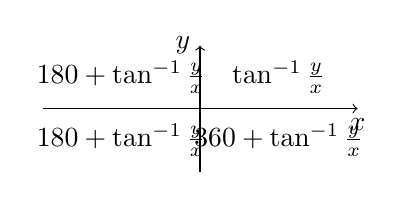
\begin{tikzpicture}
            % Achsen 
            \draw [->] (-2, 0) -- (2, 0) node [below] {$x$};
            \draw [->] (0, -0.8) -- (0, 0.8) node [left] {$y$};
            % Formeln
            \node at ( 1,  0.4) {$\tan^{-1}\frac{y}{x}$};
            \node at ( 1, -0.4) {$360\degree + \tan^{-1}\frac{y}{x}$};
            \node at (-1, -0.4) {$180\degree + \tan^{-1}\frac{y}{x}$};
            \node at (-1,  0.4) {$180\degree + \tan^{-1}\frac{y}{x}$};
        \end{tikzpicture}
    \end{center}
\end{minipage}

\myul{\textbf{Kartesisch $\rightarrow$ Sphärisch:}}\\
Word

\myul{\textbf{Zylindrisch $\rightarrow$ Kartesisch:}}\\
Word

\myul{\textbf{Zylindrisch $\rightarrow$ Sphärisch:}}\\
Word

\myul{\textbf{Sphärisch $\rightarrow$ Kartesisch:}}\\
Word

\myul{\textbf{Sphärisch $\rightarrow$ Zylindrisch:}}\\
Word

\subsection{Längenintegrale}
\subsubsection{Längenelemente}
$ (\diff l)^2 = (\diff x)^2 + (\diff y)^2 + (\diff z)^2 = \dots $
\subsubsection{Länge einer Funktion}
$ \int\limits_{L} f(x,y,z) \diff l = \dots $

\subsection{Flächenintegrale}
\subsubsection{Flächenelemente}
$ \diff s = f(\diff x, \diff y, \diff z) = \dots $
\subsubsection{Flächeninhalt einer Oberfläche}
$ \int\limits_{S} f(x,y,z) \diff s = \dots $

\subsection{Volumenintegrale}
\subsubsection{Volumenelemente}
$ \diff s = f(\diff x, \diff y, \diff z) = \dots $
\subsubsection{Volumen eines Körpers}
$ \int\limits_{V} f(x,y,z) \diff v = \dots $

\subsection{Anwendungen Trippel-Integrale}
\resizebox{\linewidth}{!}{
    \begin{tabular}{|l|l|l|l|}  
        \hline
        \bf{Allgemein} & \bf{Kartesische Koordinaten} & \bf{Zylinderkoordinaten} & \bf{Kugelkoordinaten} \\
        \hline
        \multicolumn{4}{|l|}{\bf{Beispiel}} \\
        \hline
        $ A = \int\limits_{A} \diff a $ & 
        $ = \int\limits_{X}\int\limits_{Y}\int\limits_{Z} \diff z \diff y \diff x $ &
        $ = \dots $ &
        $ = \dots $ \\
        \hline
    \end{tabular}
}
\smallskip